\section{\tl{Application of MCA to the genetic data along with OPNMF to the imaging data}}
\en{Combining the two previous techniques, we now apply MCA to the genetic data, and OPNMF to the imaging data, and combine the two transformed views for the classification task. 
}
\subsection{\en{Without scaling or balancing:}}
\en{
\begin{figure}[H]
    \centering
    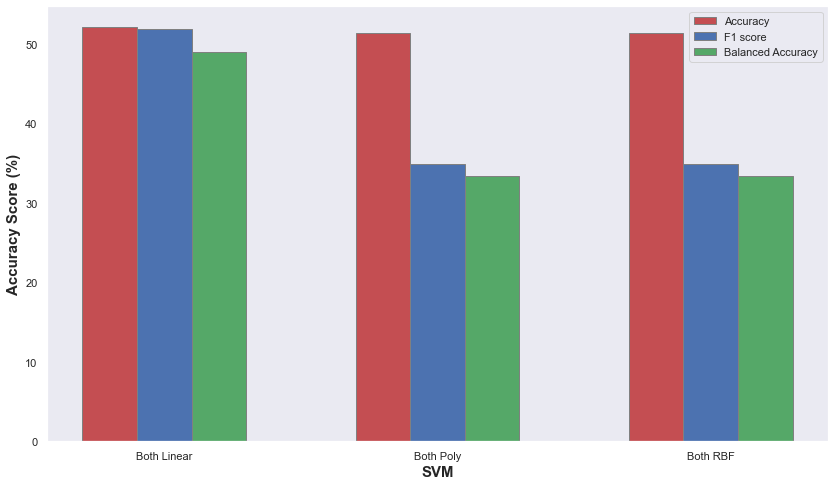
\includegraphics[width=\textwidth]{figures/Results/MCA_NMF/MCA_NMF_out.png}
    \caption[\en{MCA OPNMF Classification metrics}]{\en{Classification metric using both views (imaging and genetic) on the SVM kernels (Linear, Polynomial, RBF), using the MCA transformed genetic and OPNMF transformed imaging data.}}
\end{figure}

% \begin{figure}[H]
%     \centering
%     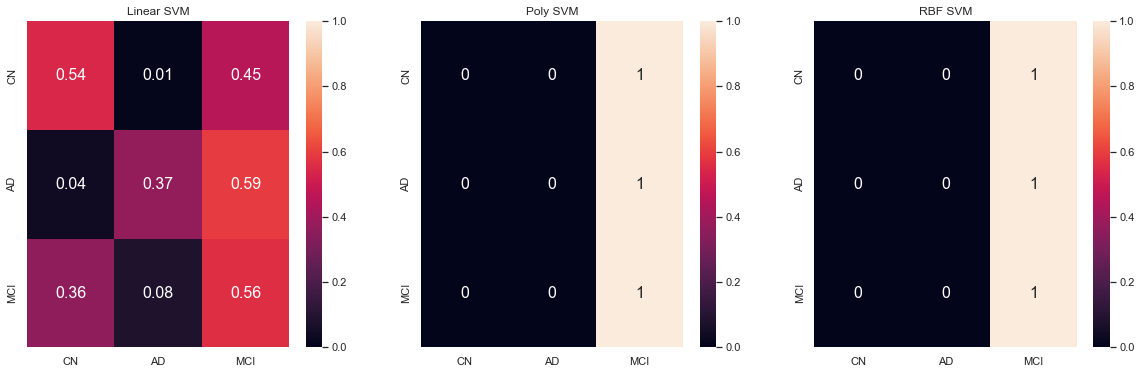
\includegraphics[width=\textwidth]{figures/Results/MCA_NMF/MCA_NMF_CM_out.png}
%     \caption[\en{MCA OPNMF Confusion Matrices}]{\en{The Confusion Matrices for each class, per SVM kernel, for the MCA transformed genetic and OPNMF transformed imaging data.}}
% \end{figure}

\begin{figure}[H]
    \centering
    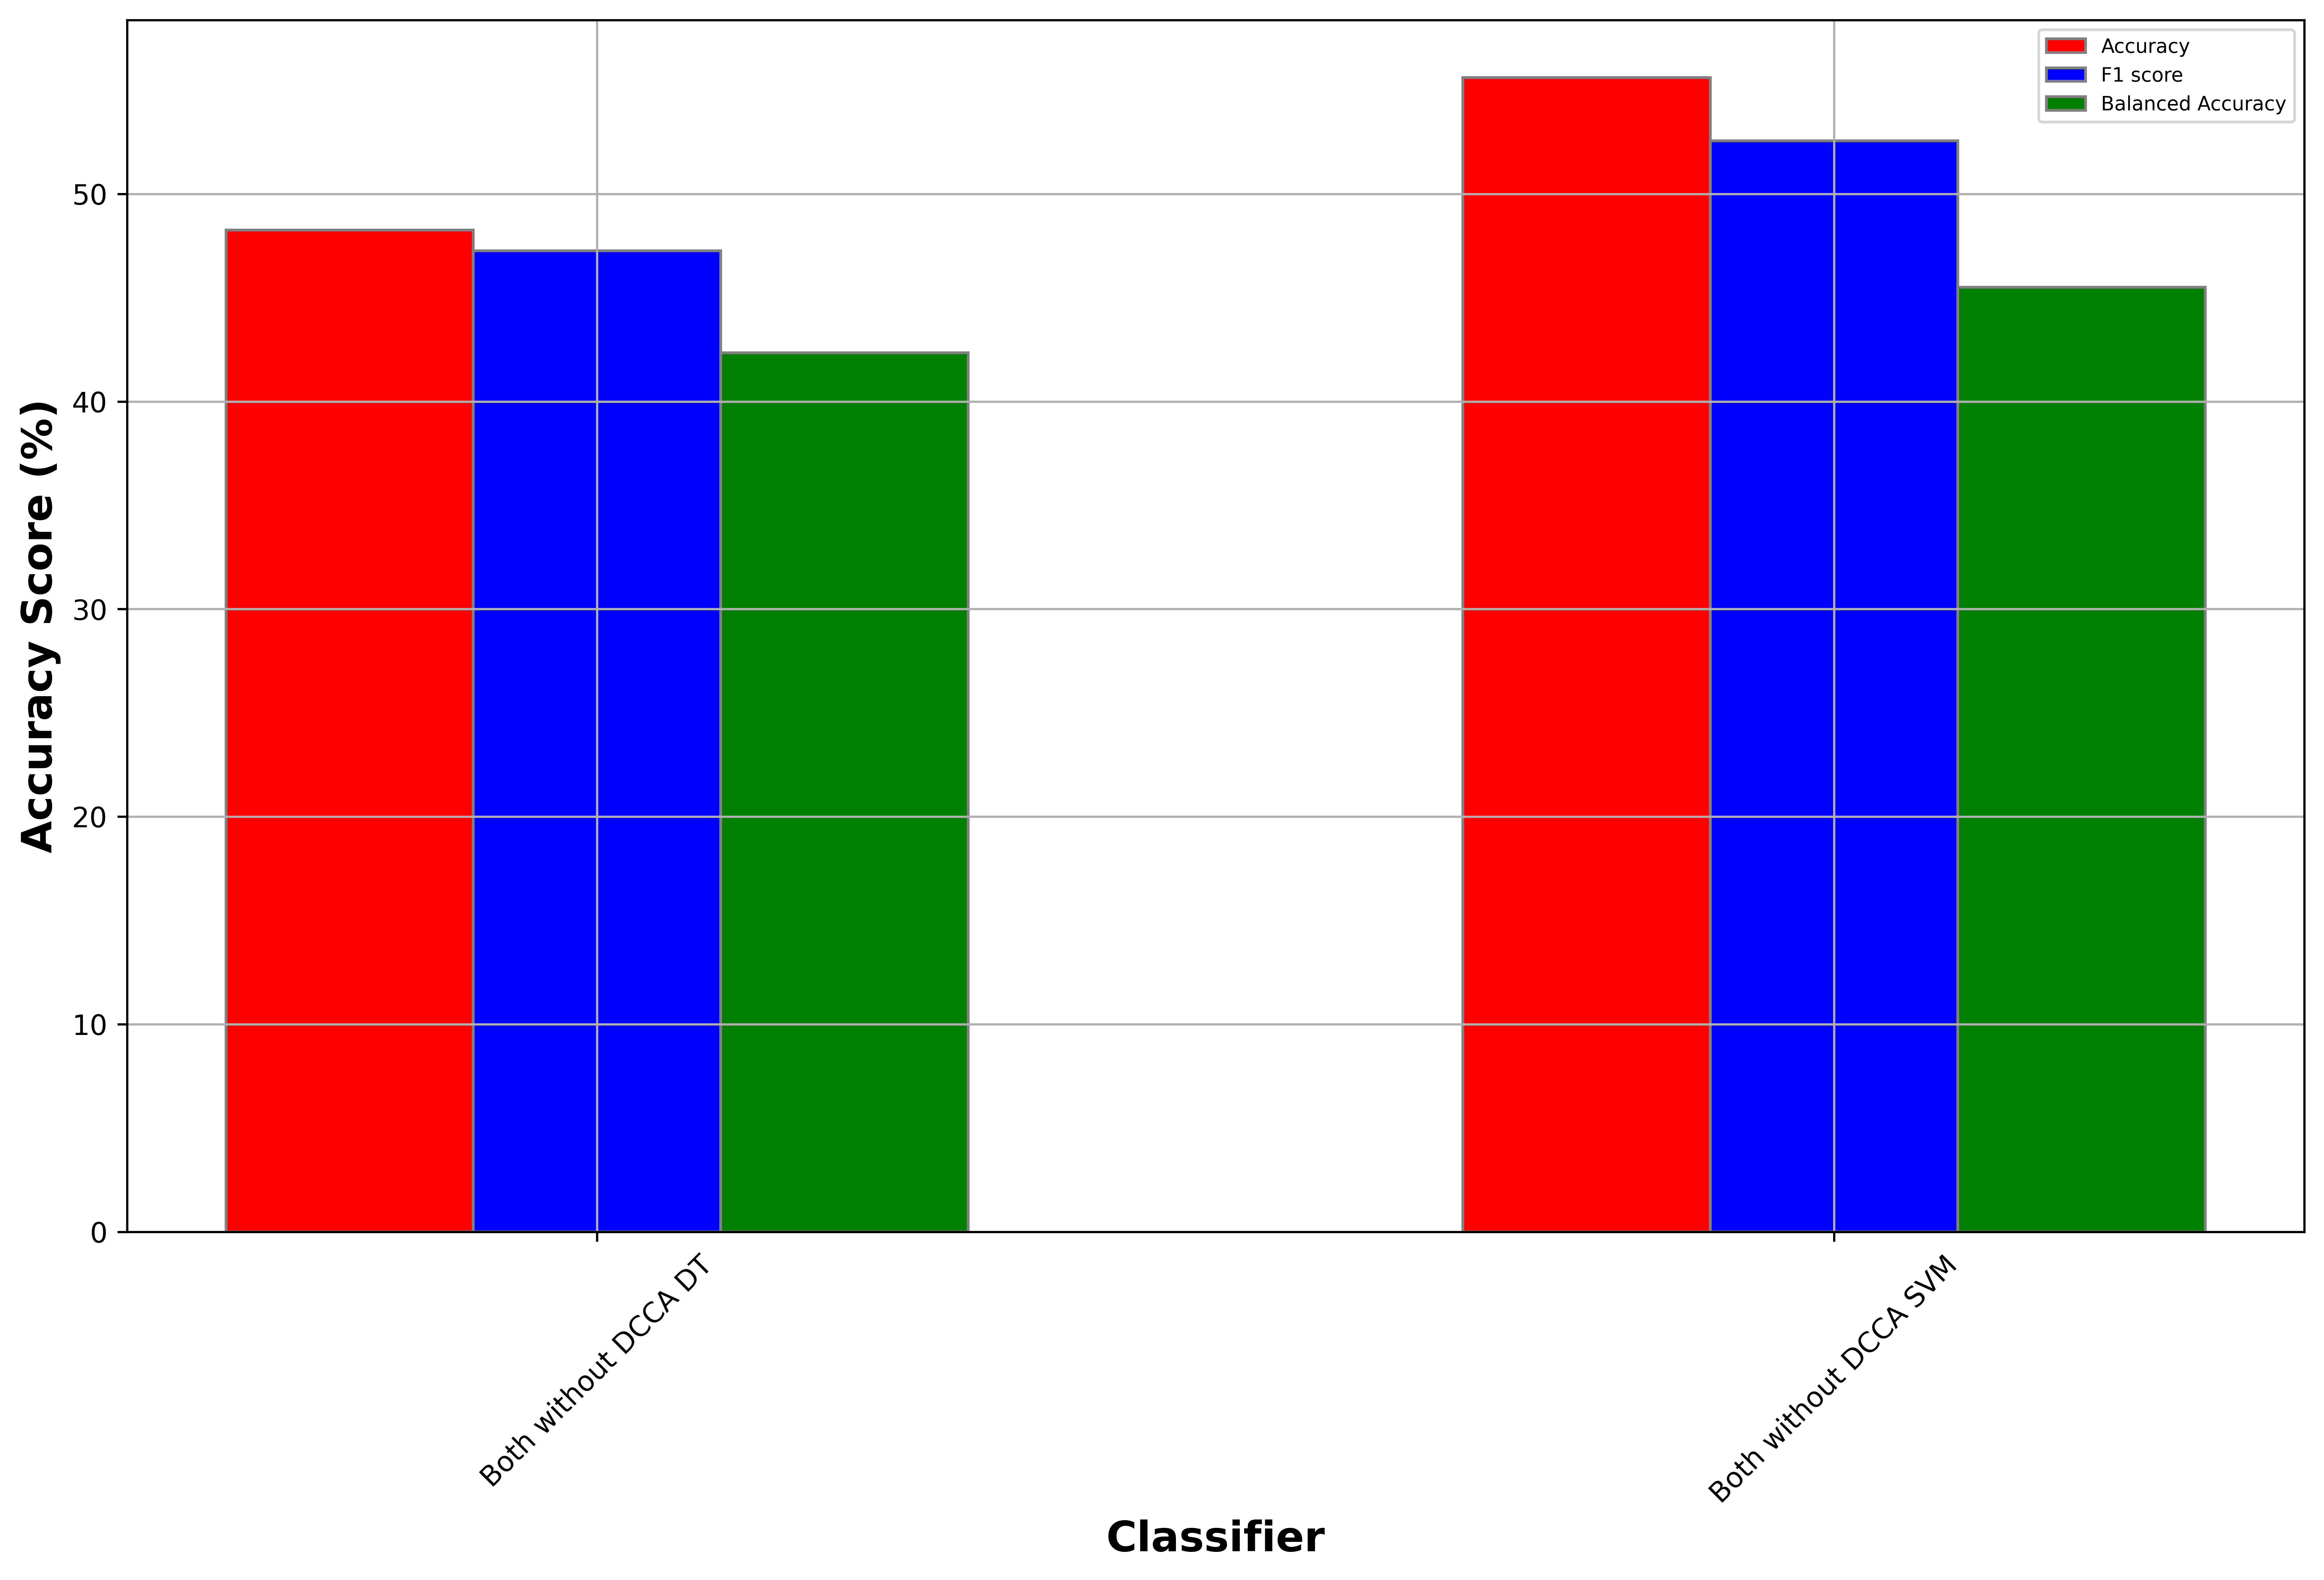
\includegraphics[width=\textwidth]{figures/Results/MCA_NMF/Bagging_MCAOPNMF_out.png}
    \caption[\en{MCA and OPNMF Bagging Classification metrics}]{\en{Classification metric using Bagging on the MCA and OPNMF transformed imaging and genetic data.}}
\end{figure}

% \begin{figure}[H]
%     \centering
%     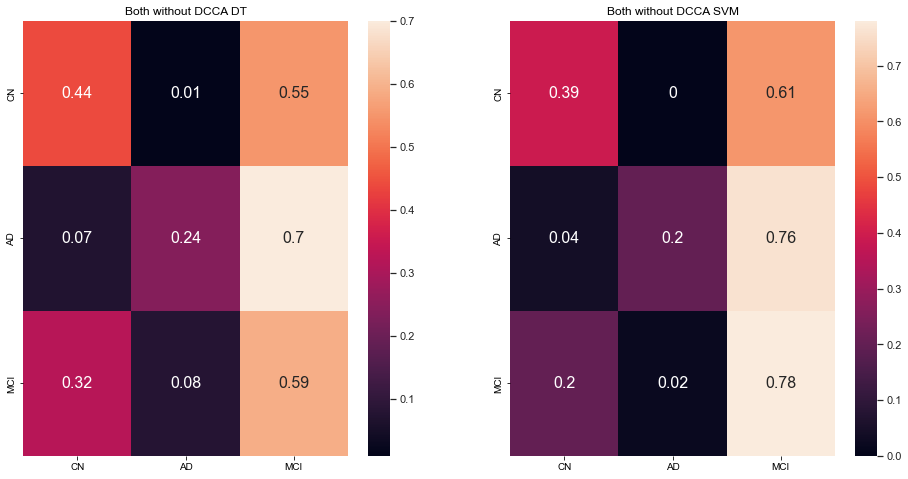
\includegraphics[width=\textwidth]{figures/Results/MCA_NMF/Bagging_MCAOPNMF_CM_out.png}
%     \caption[\en{MCA and OPNMF Bagging Confusion Matrices}]{\en{The Confusion Matrices for each class, with Bagging, for the MCA and OPNMF transformed imaging and genetic data.}}
% \end{figure}

\begin{figure}[H]
    \centering
    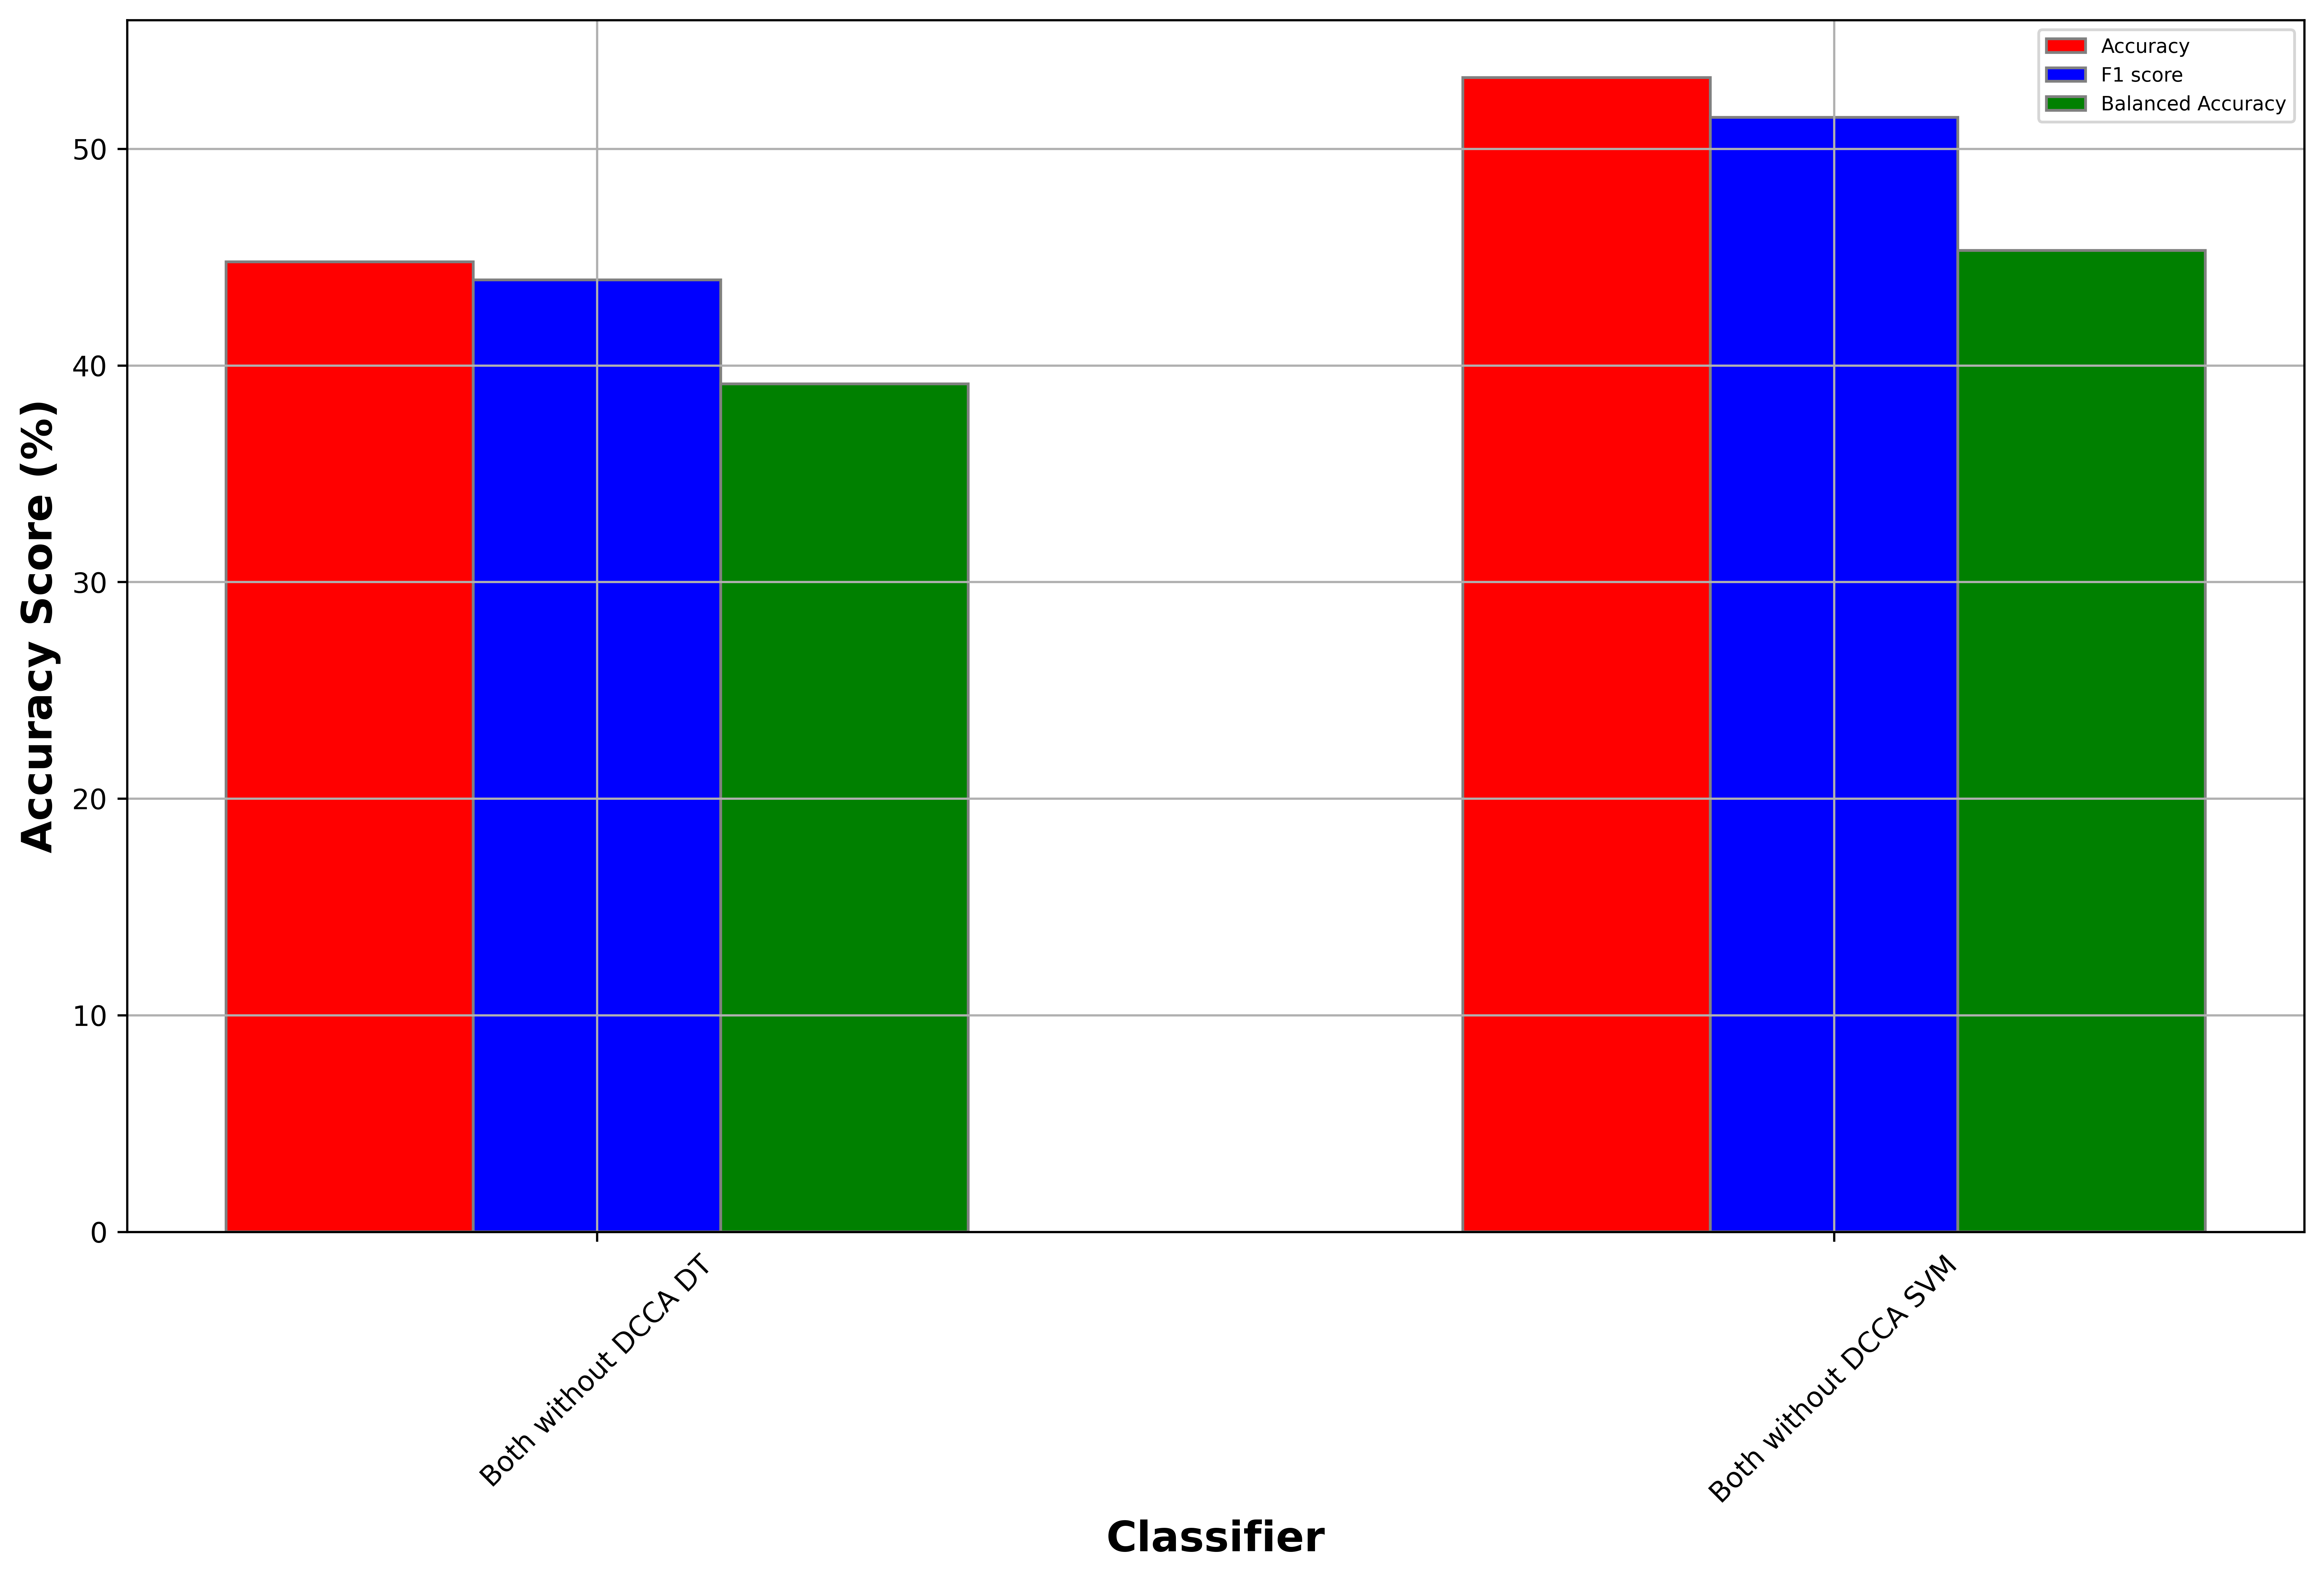
\includegraphics[width=\textwidth]{figures/Results/MCA_NMF/AdaBoost_MCAOPNMF_out.png}
    \caption[\en{MCA and OPNMF AdaBoost Classification metrics}]{\en{Classification metric using AdaBoost on the MCA and OPNMF transformed imaging and genetic data.}}
\end{figure}

% \begin{figure}[H]
%     \centering
%     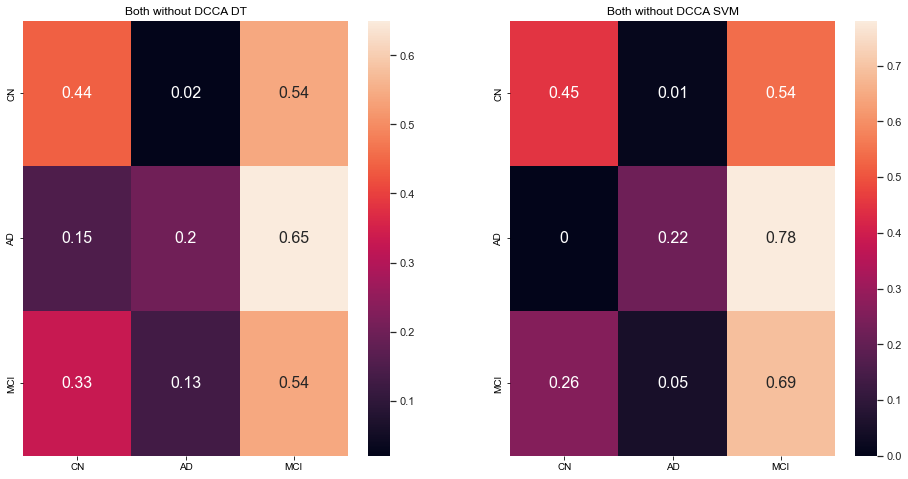
\includegraphics[width=\textwidth]{figures/Results/MCA_NMF/AdaBoost_MCAOPNMF_CM_out.png}
%     \caption[\en{MCA and OPNMF AdaBoost Confusion Matrices}]{\en{The Confusion Matrices for each class, with AdaBoost, for the MCA and OPNMF transformed imaging and genetic data.}}
% \end{figure}


}
\subsection{\en{With scaling and balancing:}}
\en{
\begin{figure}[H]
    \centering
    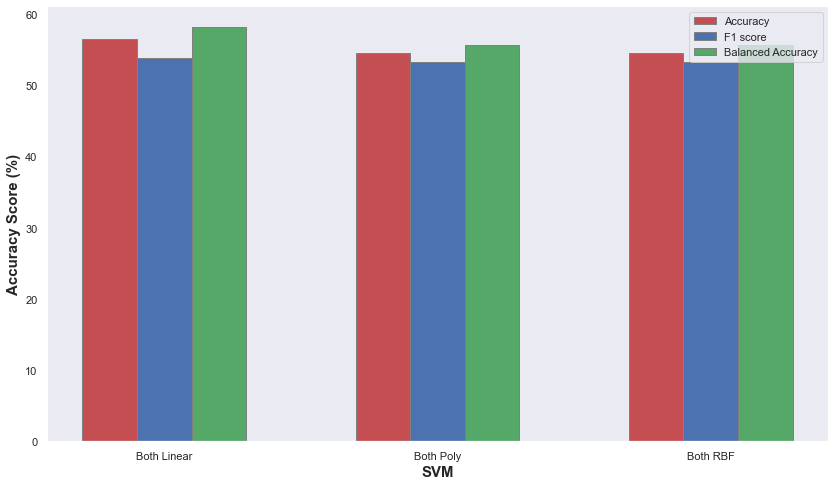
\includegraphics[width=\textwidth]{figures/Results/MCA_NMF/MCA_NMF_with.png}
    \caption[\en{MCA OPNMF Classification metrics with scaling and balancing}]{\en{Classification metric using both views (imaging and genetic) on the SVM kernels (Linear, Polynomial, RBF), using the MCA transformed genetic and OPNMF transformed imaging data.}}
\end{figure}

% \begin{figure}[H]
%     \centering
%     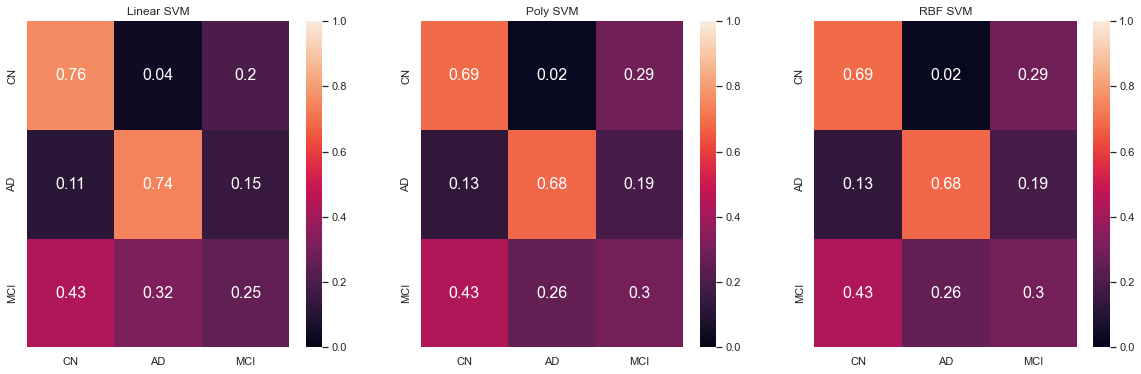
\includegraphics[width=\textwidth]{figures/Results/MCA_NMF/MCA_NMF_CM_with.png}
%     \caption[\en{MCA OPNMF Confusion Matrices with scaling and balancing}]{\en{The Confusion Matrices for each class, per SVM kernel, for the MCA transformed genetic and OPNMF transformed imaging data.}}
% \end{figure}

\begin{figure}[H]
    \centering
    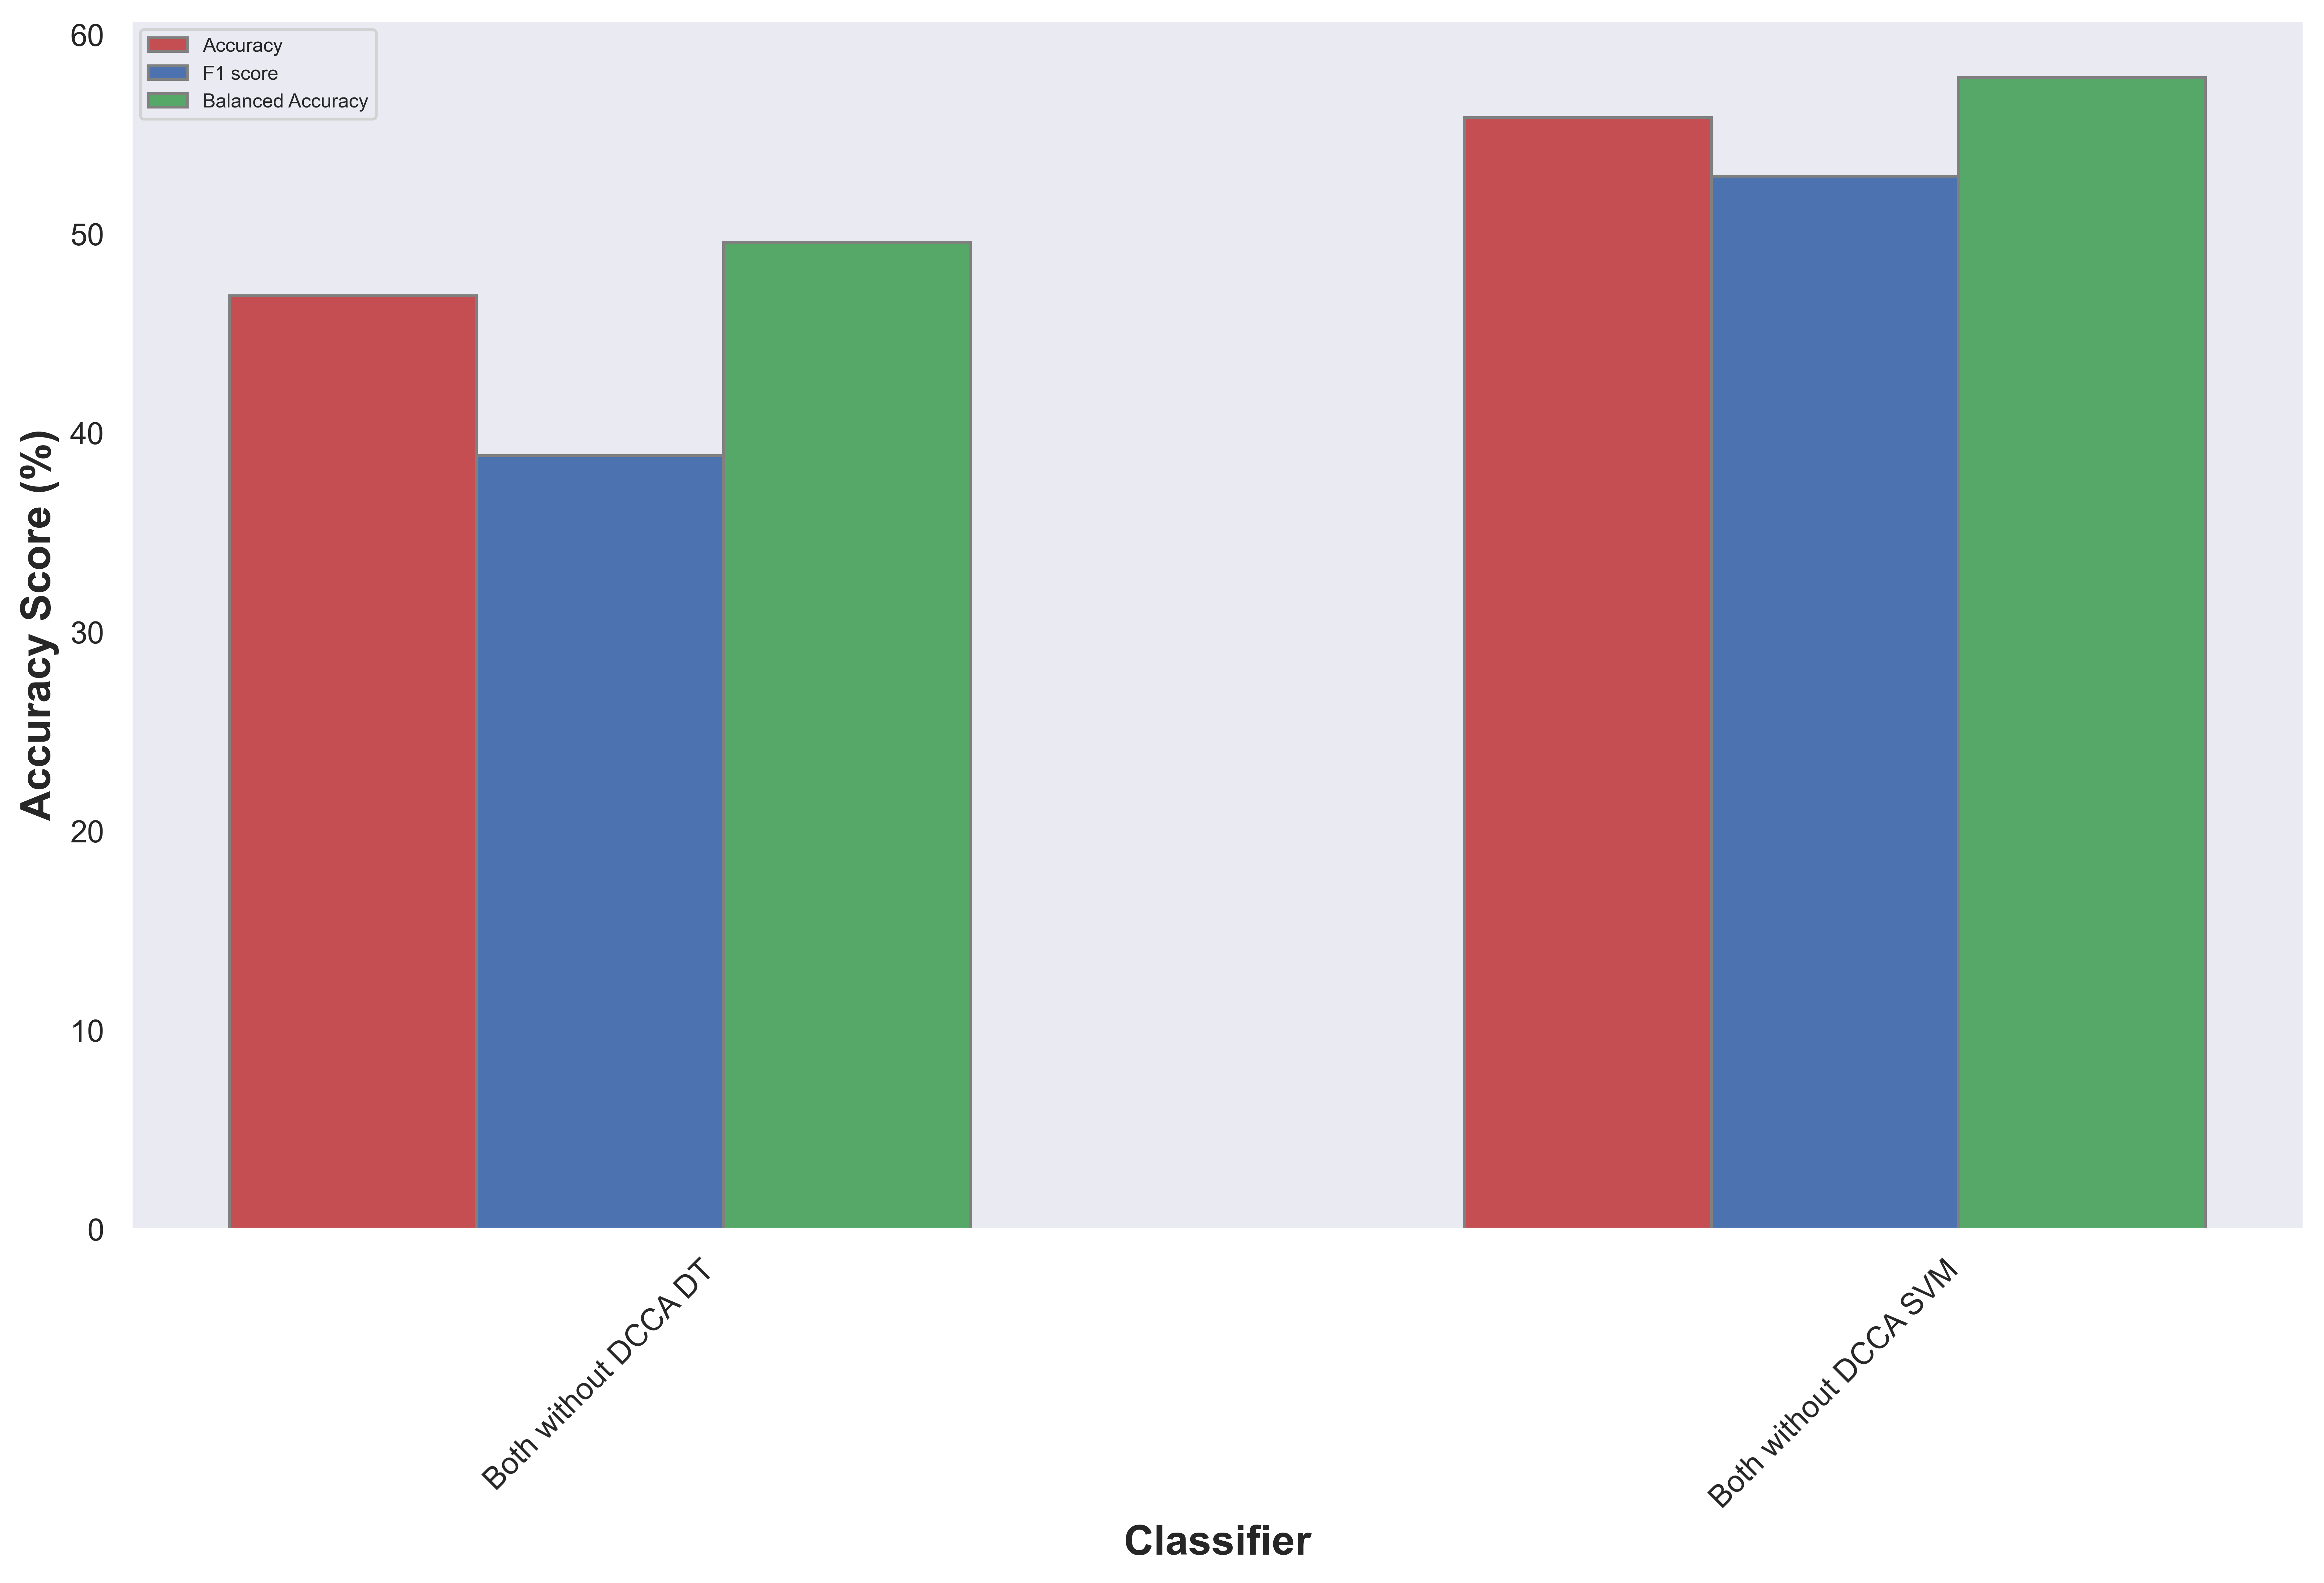
\includegraphics[width=\textwidth]{figures/Results/MCA_NMF/Bagging_MCAOPNMF_with.png}
    \caption[\en{MCA and OPNMF Bagging Classification metrics with scaling and balancing}]{\en{Classification metric using Bagging on the MCA and OPNMF transformed imaging and genetic data.}}
\end{figure}

% \begin{figure}[H]
%     \centering
%     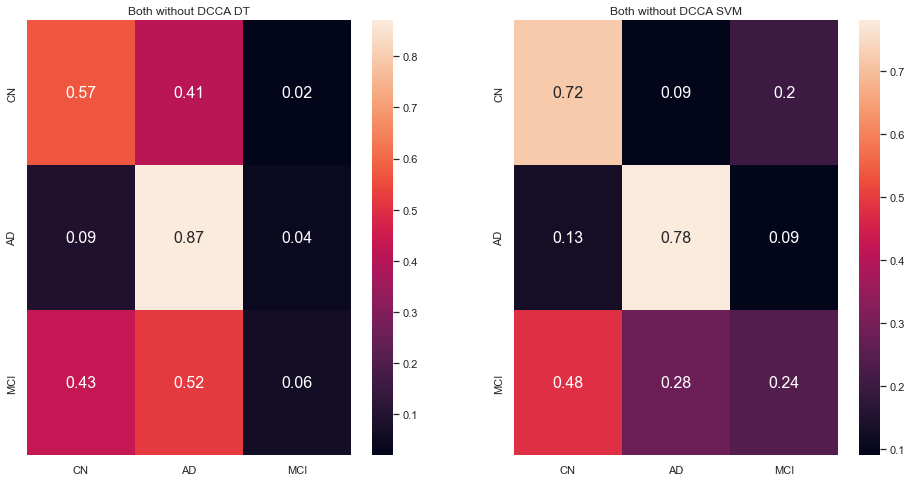
\includegraphics[width=\textwidth]{figures/Results/MCA_NMF/Bagging_MCAOPNMF_CM_with.png}
%     \caption[\en{MCA and OPNMF Bagging Confusion Matrices with scaling and balancing}]{\en{The Confusion Matrices for each class, with Bagging, for the MCA and OPNMF transformed imaging and genetic data.}}
% \end{figure}

\begin{figure}[H]
    \centering
    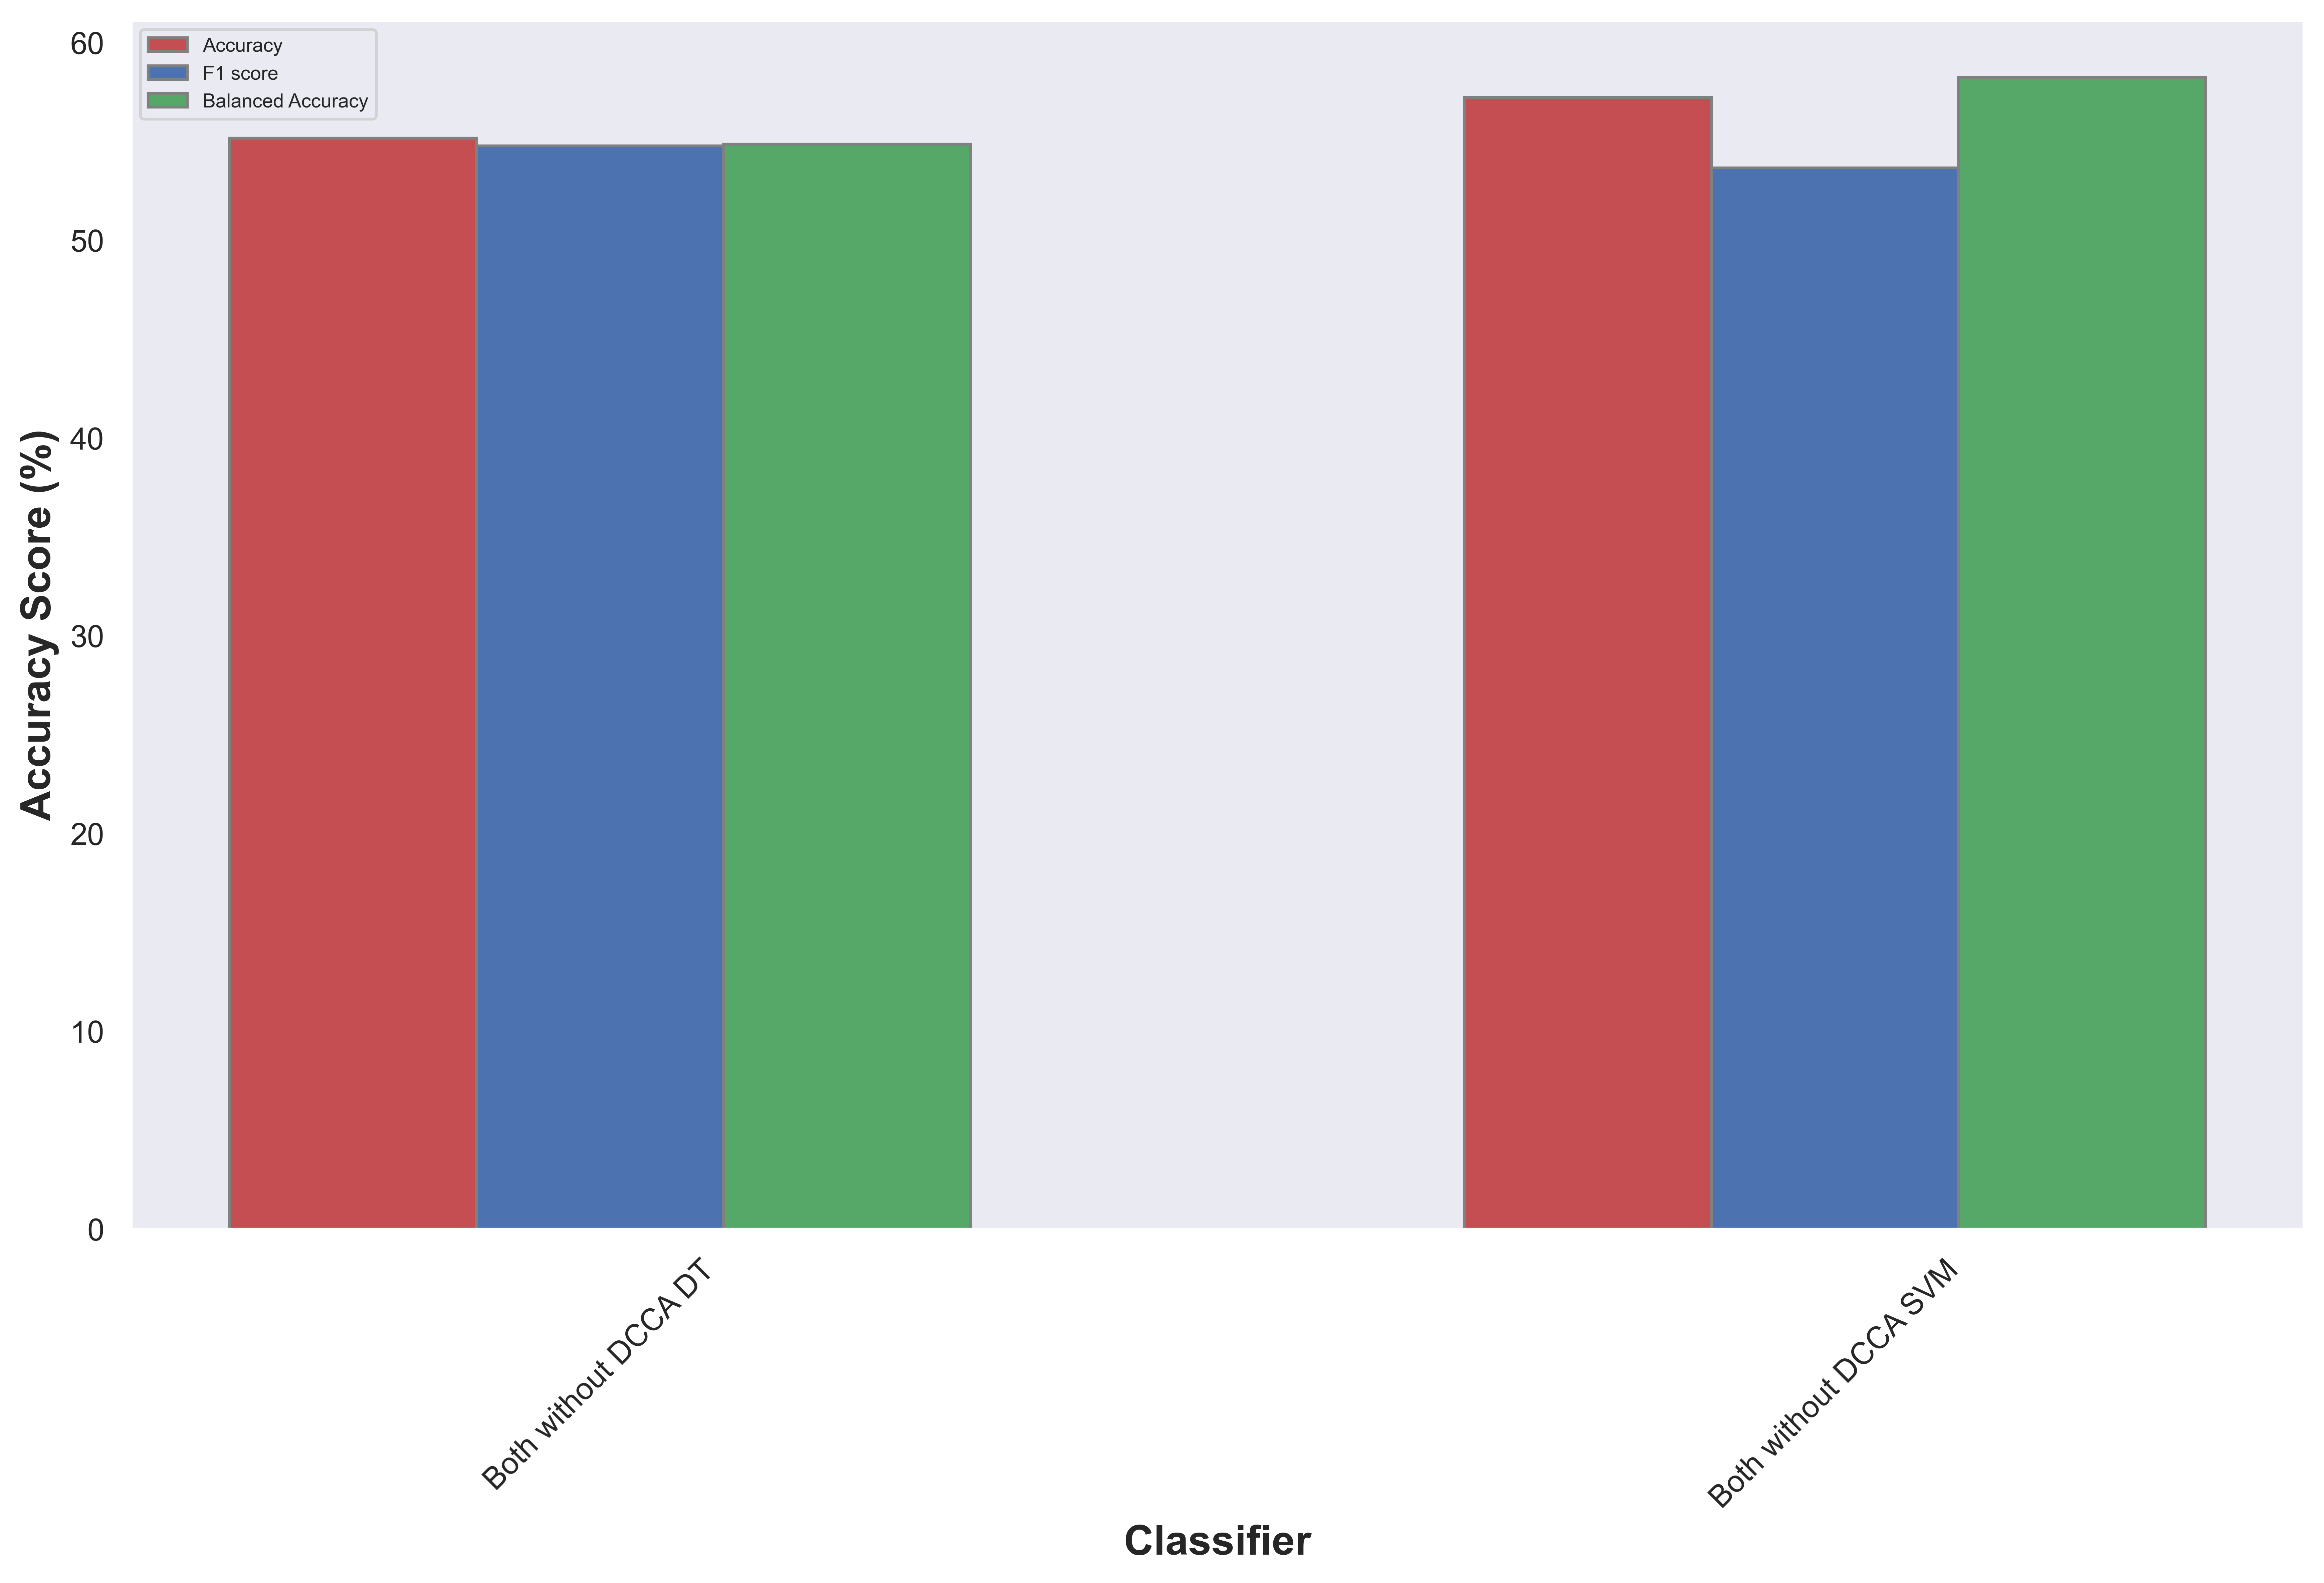
\includegraphics[width=\textwidth]{figures/Results/MCA_NMF/AdaBoost_MCAOPNMF_with.png}
    \caption[\en{MCA and OPNMF AdaBoost Classification metrics with scaling and balancing}]{\en{Classification metric using AdaBoost on the MCA and OPNMF transformed imaging and genetic data.}}
\end{figure}

% \begin{figure}[H]
%     \centering
%     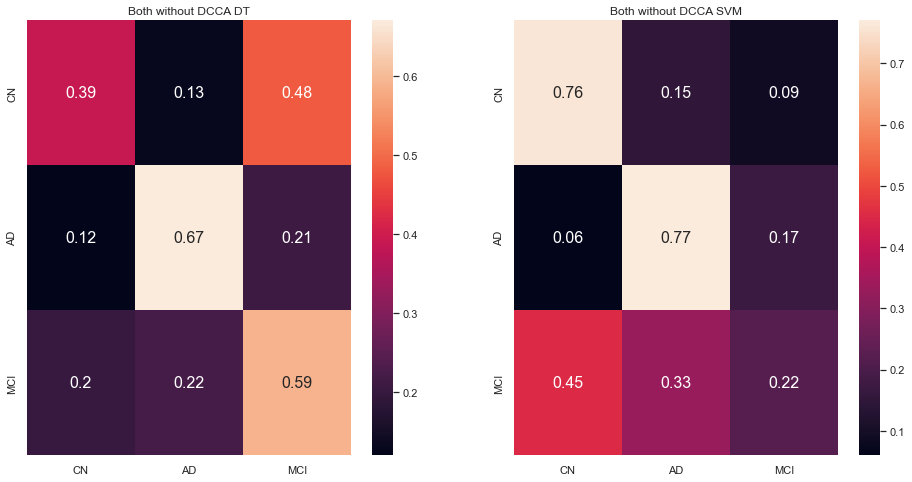
\includegraphics[width=\textwidth]{figures/Results/MCA_NMF/AdaBoost_MCAOPNMF_CM_with.png}
%     \caption[\en{MCA and OPNMF AdaBoost Confusion Matrices with scaling and balancing}]{\en{The Confusion Matrices for each class, with AdaBoost, for the MCA and OPNMF transformed imaging and genetic data.}}
% \end{figure}

The following tables present the complete results for the MCA and OPNMF transformed data, for each model, for each metric, for each view, and either with or without scaling and balancing. With green are highlighted the best values for each metric, depending on whether scaling and balancing were applied:

\begin{figure} [H]
    \centering
    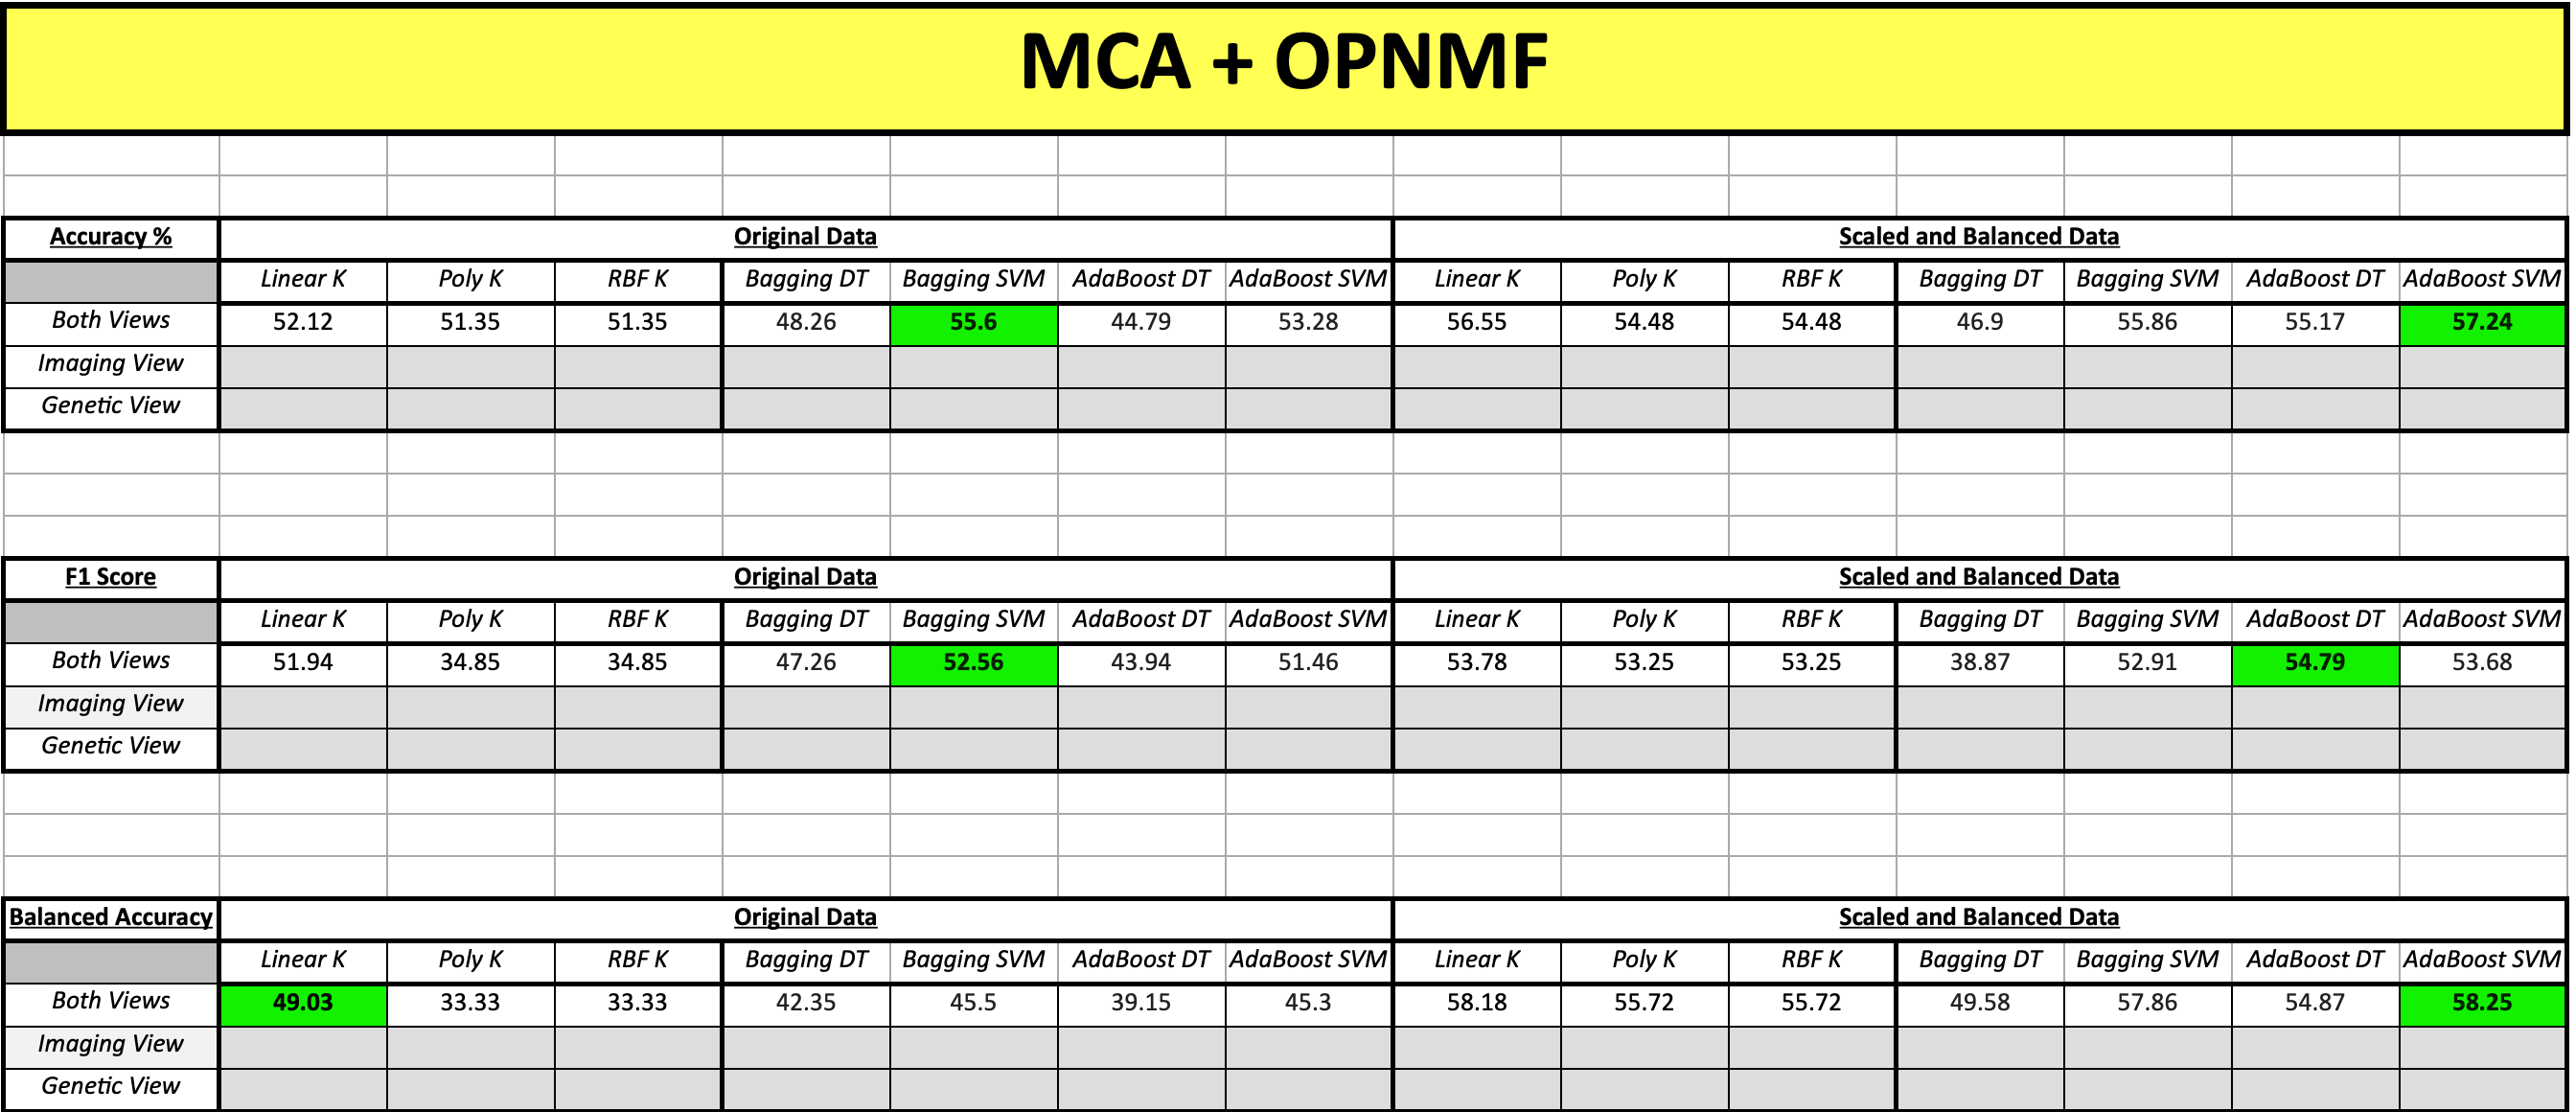
\includegraphics[width=\textwidth]{figures/Results/Analytical_Table_MCA_OPNMF.png}
    \caption[\en{Analytical table of results for MCA OPNMF data classification}]{\en{For each model and classifier, the metric scores for MCA and OPNMF transformed data classification are presented. Highlighted green are the best performing models, for each metric.}}
    \label{fig: Summary Table for classification scores for MCA - OPNMF transformed data}
\end{figure}
}